\chapter{Implementation and Results} \label{ch:implementation}
rgrtgrtgrgtrgrrg

\section{Android Application}
sdfdsfdsfds

Sensors

GNSS, with projection to Magna-Sirgas
Barometer
Attitude
\section{Ground Control Station}
sdfsdfdsd

\section{LQI Controller Implementation}
grtgrgtrgtrgtrg

\subsection{Stabilize Mode (LQI)}
grtgtrgrtgrg

\begin{figure}[H]
\begin{subfigure}{.5\linewidth}
\centering
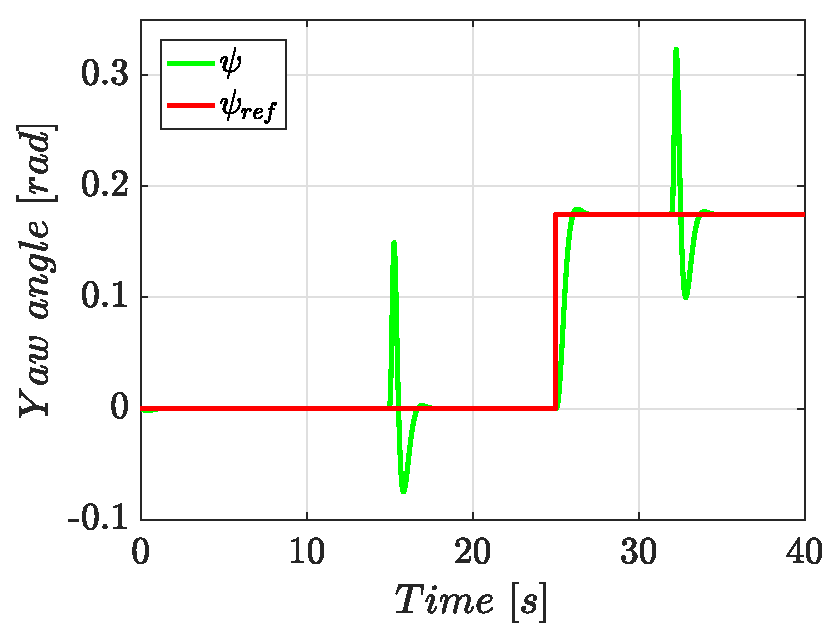
\includegraphics[width=7.0cm]{stabilize_psi_lqi}
\caption{Rotation about $x$ axis, $J_{xx}$ experiment}
\label{fig:stabilize_psi_lqi_imp}
\end{subfigure}%
\begin{subfigure}{.5\linewidth}
\centering
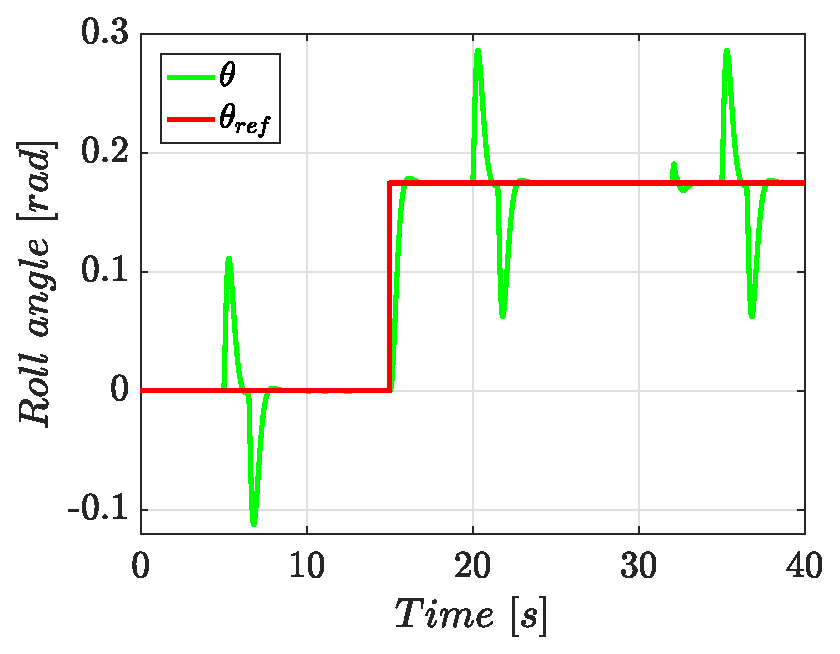
\includegraphics[width=7.0cm]{stabilize_theta_lqi}
\caption{Rotation about $y$ axis, $J_{yy}$ experiment}
\label{fig:stabilize_theta_lqi_imp}
\end{subfigure}\\[1ex]
\begin{subfigure}{\linewidth}
\centering
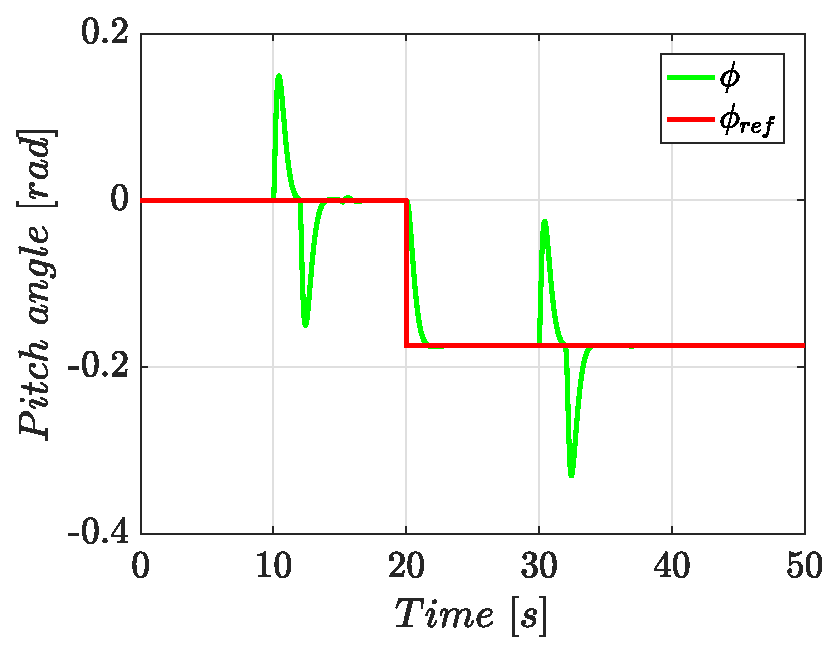
\includegraphics[width=7.0cm]{stabilize_phi_lqi}
\caption{Rotation about $z$ axis, $J_{zz}$ experiment}
\label{fig:stabilize_psi_lqi_imp}
\end{subfigure}
\caption{Rotation about $x$, $y$ and $z$ axes during the bifilar pendulum experiments}
\label{fig:stabilize_lqi_imp}
\end{figure}

\subsection{Altitude Hold Mode (LQI)}
trgrgrtgtrgr

\begin{figure}[H]
\begin{subfigure}{.5\linewidth}
\centering
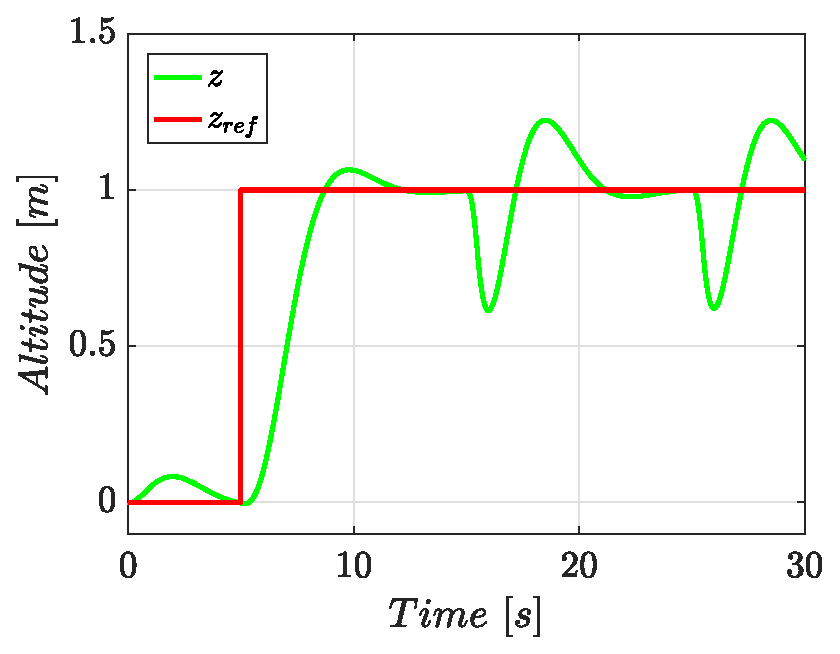
\includegraphics[width=7.0cm]{althold_z_lqi}
\caption{Rotation about $x$ axis, $J_{xx}$ experiment}
\label{fig:althold_z_lqi}
\end{subfigure}%
\begin{subfigure}{.5\linewidth}
\centering
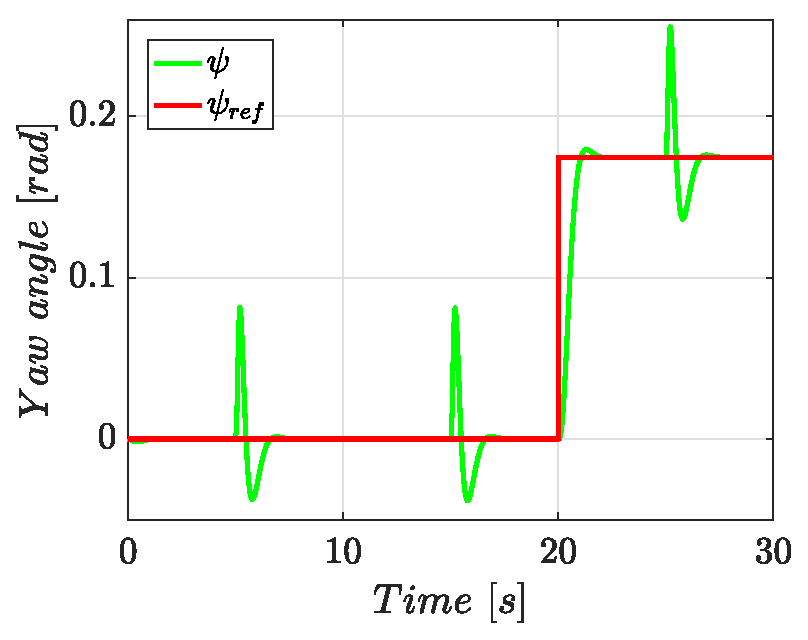
\includegraphics[width=7.0cm]{althold_psi_lqi}
\caption{Rotation about $y$ axis, $J_{yy}$ experiment}
\label{fig:althold_psi_lqi}
\end{subfigure}\\[1ex]
\begin{subfigure}{0.5\linewidth}
\centering
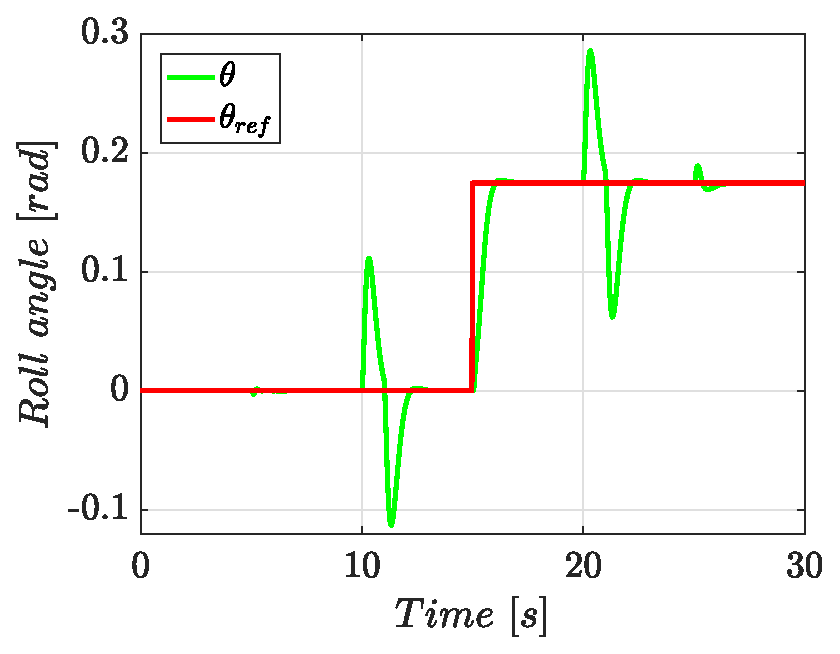
\includegraphics[width=7.0cm]{althold_theta_lqi}
\caption{Rotation about $z$ axis, $J_{zz}$ experiment}
\label{fig:althold_theta_lqi}
\end{subfigure}
\begin{subfigure}{0.5\linewidth}
\centering
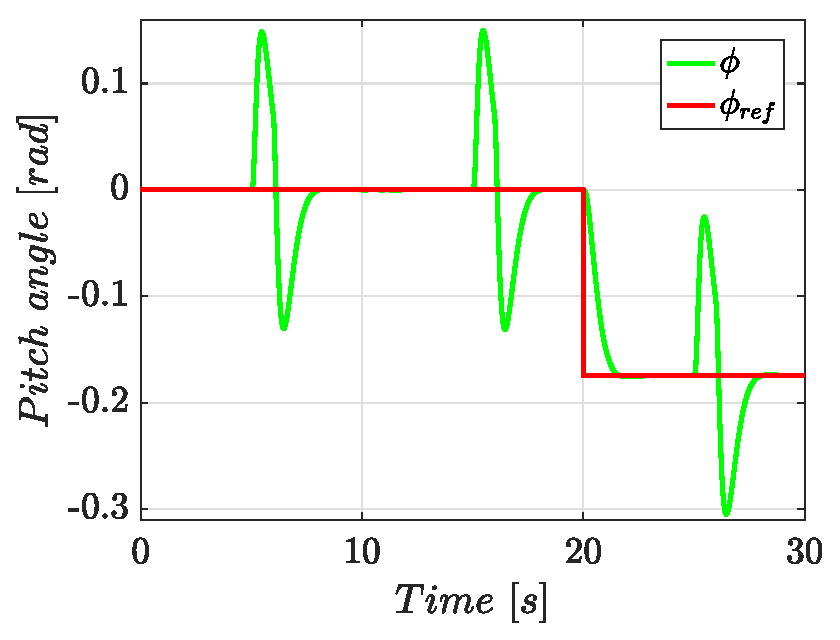
\includegraphics[width=7.0cm]{althold_phi_lqi}
\caption{Rotation about $z$ axis, $J_{zz}$ experiment}
\label{fig:althold_phi_lqi}
\end{subfigure}
\caption{Rotation about $x$, $y$ and $z$ axes during the bifilar pendulum experiments}
\label{fig:althold_lqi}
\end{figure}


\subsection{GNSS-Dependent Modes (LQI)}

\begin{figure}[h]
	\begin{center}
	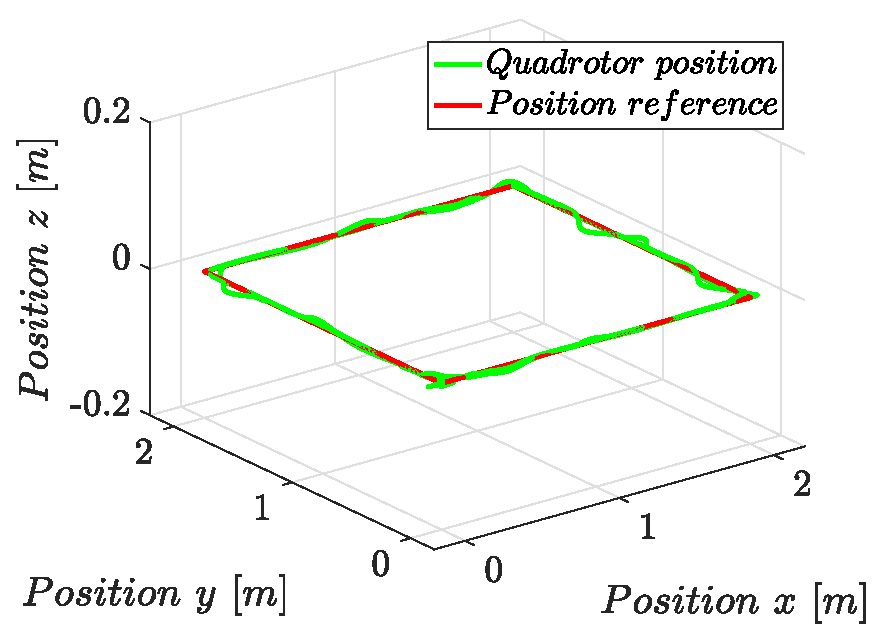
\includegraphics[width=0.8\textwidth]{auto_xyz_lqi}
	\caption{Closed-loop of the controlled system with an $H_{\infty}$ controller.}
	\label{fig:auto_xyz_lqi}
	\end{center}
	\end{figure}
	
\begin{figure}[H]
\begin{subfigure}{.5\linewidth}
\centering
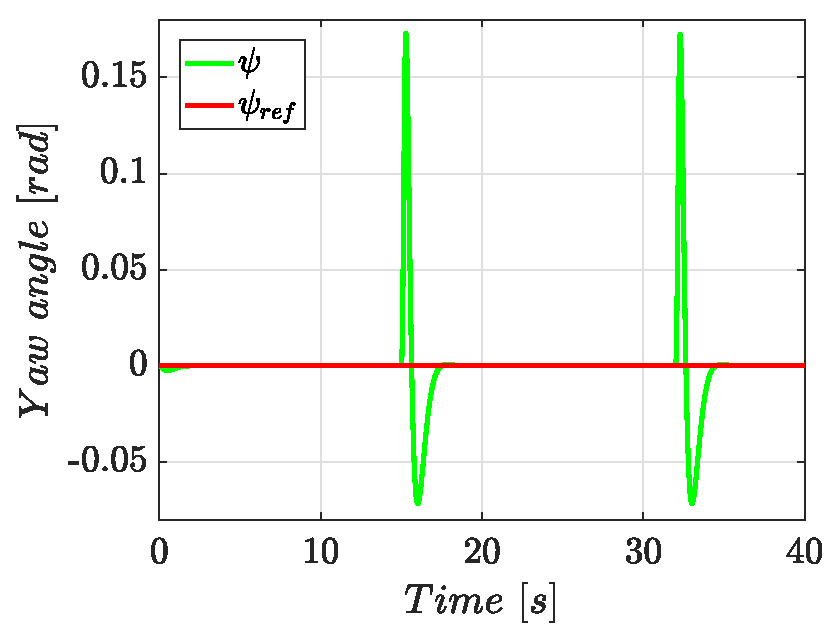
\includegraphics[width=7.0cm]{auto_psi_lqi}
\caption{Rotation about $x$ axis, $J_{xx}$ experiment}
\label{fig:auto_psi_lqi}
\end{subfigure}%
\begin{subfigure}{.5\linewidth}
\centering
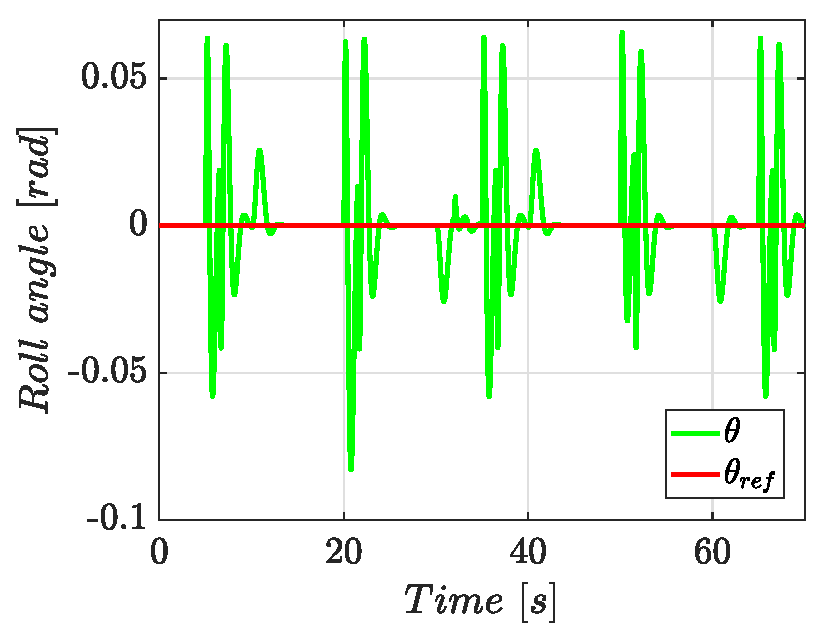
\includegraphics[width=7.0cm]{auto_theta_lqi}
\caption{Rotation about $y$ axis, $J_{yy}$ experiment}
\label{fig:auto_theta_lqi}
\end{subfigure}\\[1ex]
\begin{subfigure}{\linewidth}
\centering
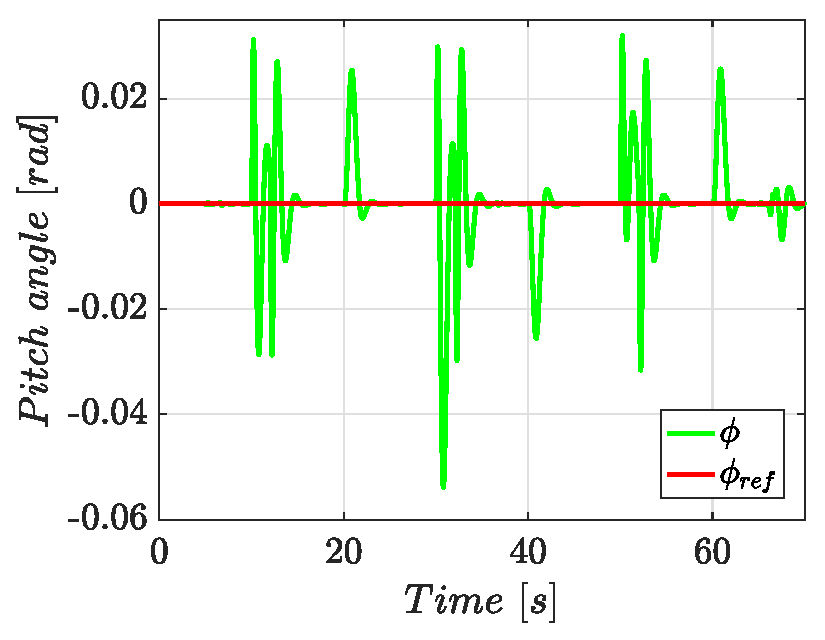
\includegraphics[width=7.0cm]{auto_phi_lqi}
\caption{Rotation about $z$ axis, $J_{zz}$ experiment}
\label{fig:auto_psi_lqi}
\end{subfigure}
\caption{Rotation about $x$, $y$ and $z$ axes during the bifilar pendulum experiments}
\label{fig:auto_lqi}
\end{figure}

\begin{figure}[h]
	\begin{center}
	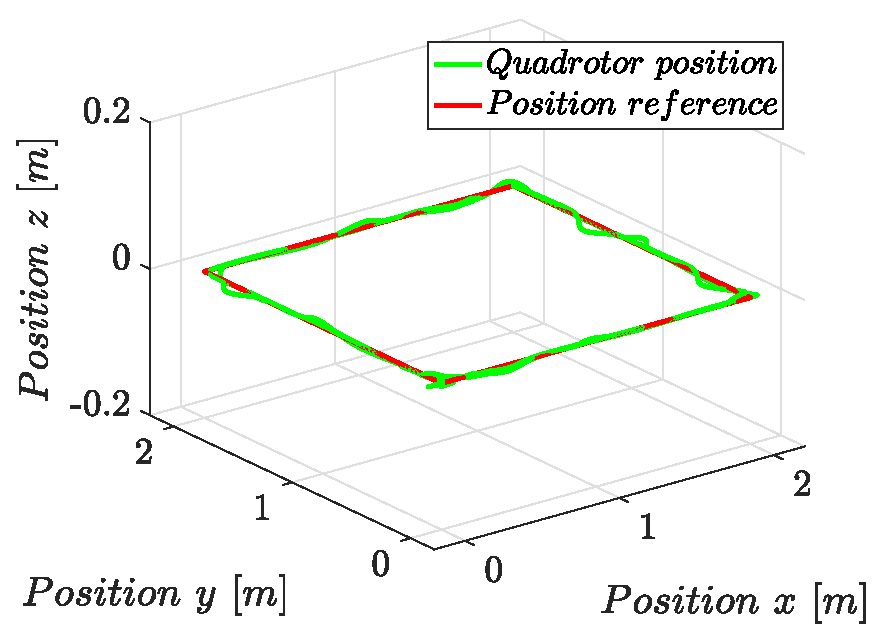
\includegraphics[width=0.8\textwidth]{auto_xyz_lqi}
	\caption{Closed-loop of the controlled system with an $H_{\infty}$ controller.}
	\label{fig:auto_xyz_lqi}
	\end{center}
	\end{figure}
	
\begin{figure}[H]
\begin{subfigure}{.5\linewidth}
\centering
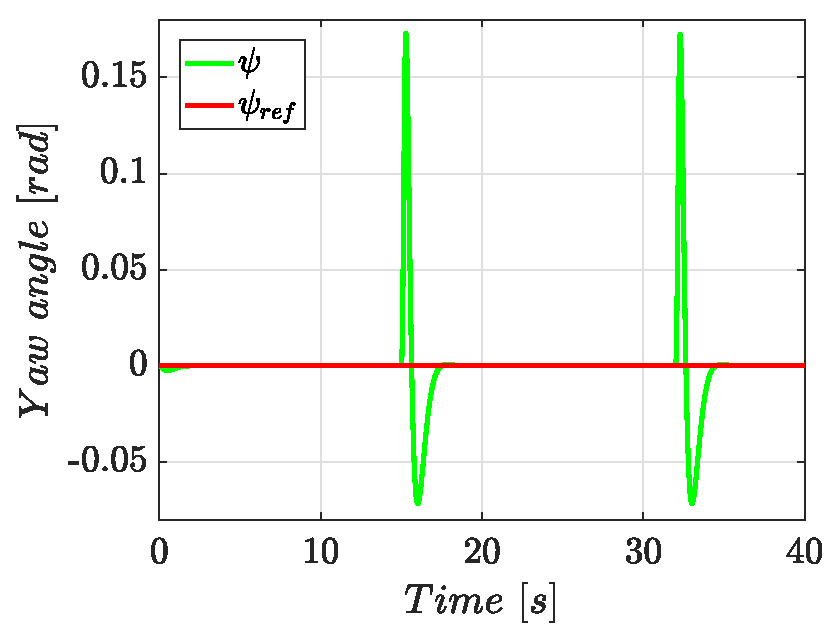
\includegraphics[width=7.0cm]{auto_psi_lqi}
\caption{Rotation about $x$ axis, $J_{xx}$ experiment}
\label{fig:auto_psi_lqi}
\end{subfigure}%
\begin{subfigure}{.5\linewidth}
\centering
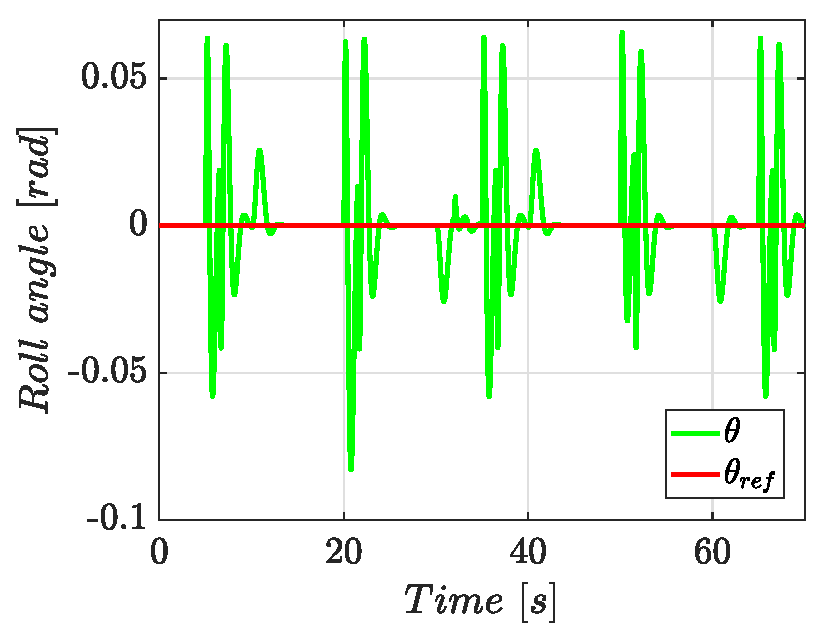
\includegraphics[width=7.0cm]{auto_theta_lqi}
\caption{Rotation about $y$ axis, $J_{yy}$ experiment}
\label{fig:auto_theta_lqi}
\end{subfigure}\\[1ex]
\begin{subfigure}{\linewidth}
\centering
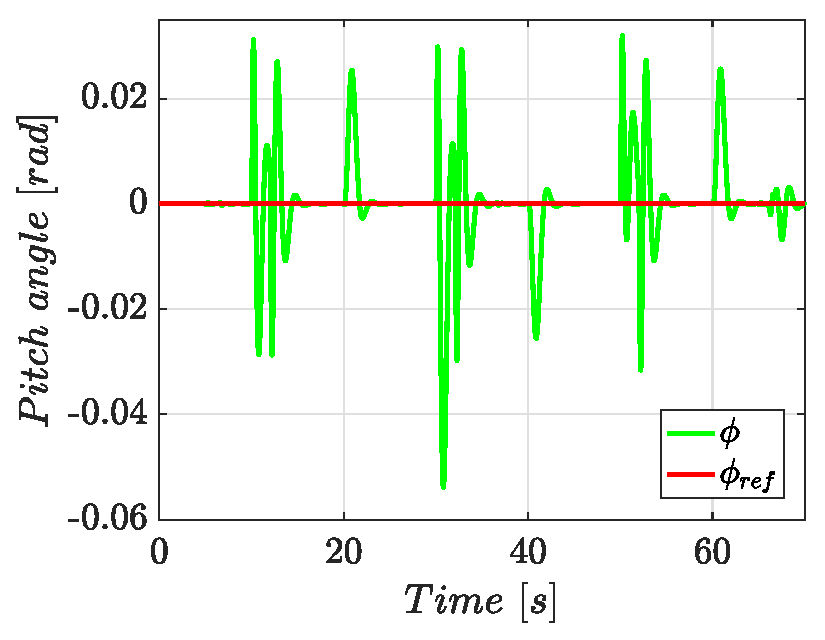
\includegraphics[width=7.0cm]{auto_phi_lqi}
\caption{Rotation about $z$ axis, $J_{zz}$ experiment}
\label{fig:auto_psi_lqi}
\end{subfigure}
\caption{Rotation about $x$, $y$ and $z$ axes during the bifilar pendulum experiments}
\label{fig:auto_lqi}
\end{figure}



\section{H$_\infty$ Controller Implementation}
grgtrgrgtrg

\subsection{Stabilize Mode (H$_\infty$)}
grtgtrgrtgrg

\begin{figure}[H]
\begin{subfigure}{.5\linewidth}
\centering
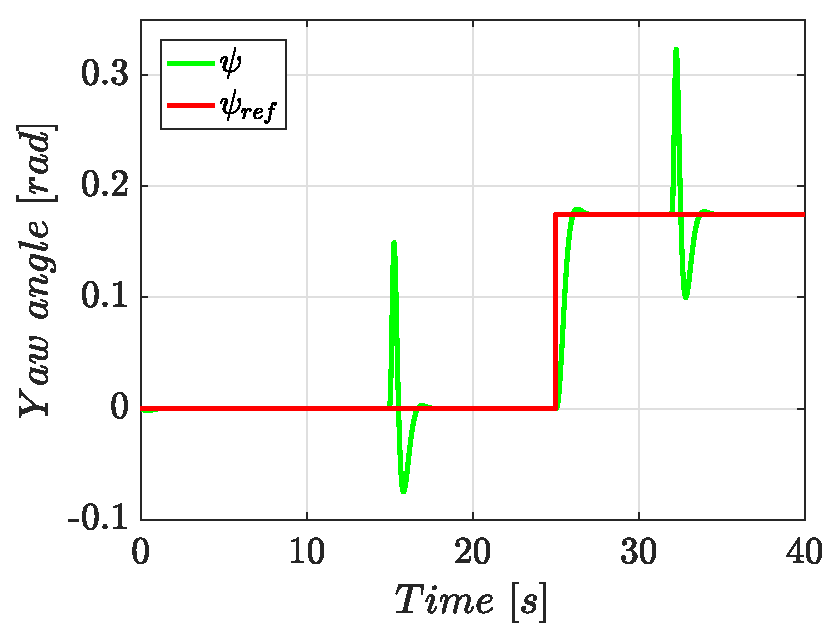
\includegraphics[width=7.0cm]{stabilize_psi_lqi}
\caption{Rotation about $x$ axis, $J_{xx}$ experiment}
\label{fig:stabilize_psi_lqi}
\end{subfigure}%
\begin{subfigure}{.5\linewidth}
\centering
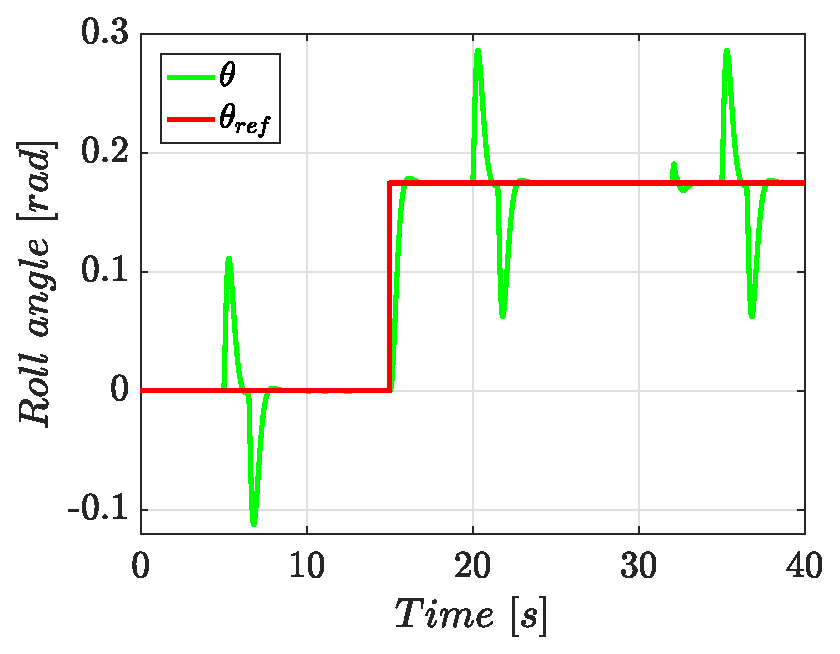
\includegraphics[width=7.0cm]{stabilize_theta_lqi}
\caption{Rotation about $y$ axis, $J_{yy}$ experiment}
\label{fig:stabilize_theta_lqi}
\end{subfigure}\\[1ex]
\begin{subfigure}{\linewidth}
\centering
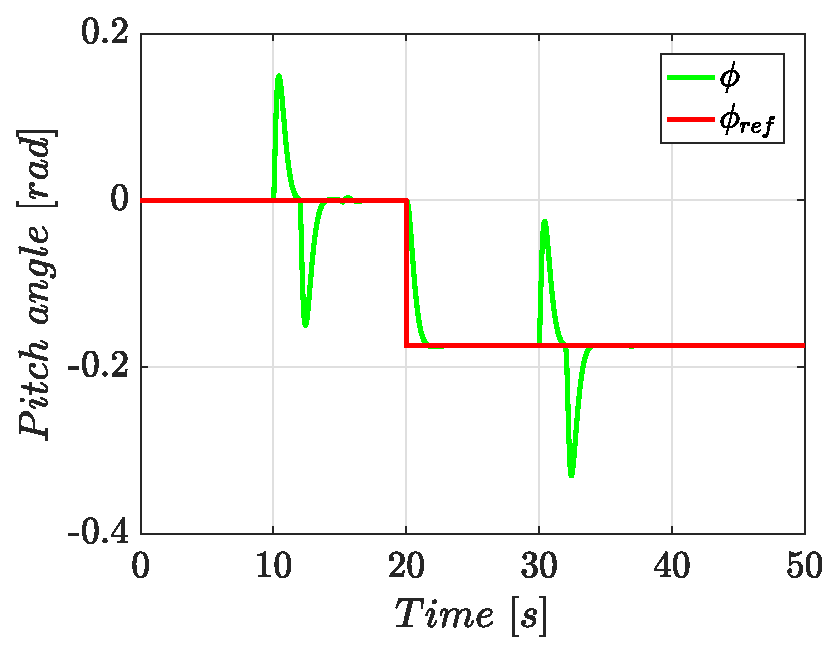
\includegraphics[width=7.0cm]{stabilize_phi_lqi}
\caption{Rotation about $z$ axis, $J_{zz}$ experiment}
\label{fig:stabilize_psi_lqi}
\end{subfigure}
\caption{Rotation about $x$, $y$ and $z$ axes during the bifilar pendulum experiments}
\label{fig:stabilize_lqi}
\end{figure}

\subsection{Altitude Hold Mode (H$_\infty$)}
trgrgrtgtrgr
\begin{figure}[H]
\begin{subfigure}{.5\linewidth}
\centering
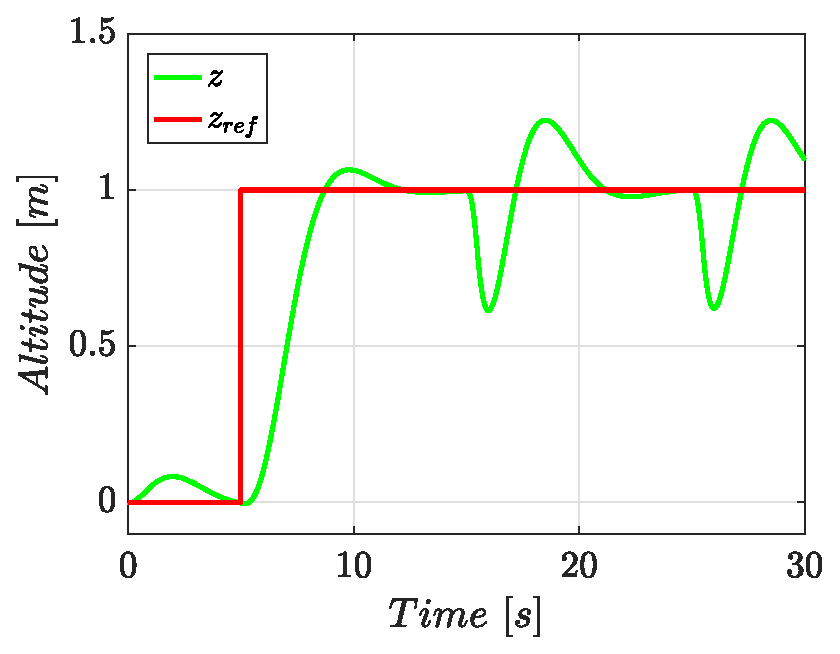
\includegraphics[width=7.0cm]{althold_z_lqi}
\caption{Rotation about $x$ axis, $J_{xx}$ experiment}
\label{fig:althold_z_lqi}
\end{subfigure}%
\begin{subfigure}{.5\linewidth}
\centering
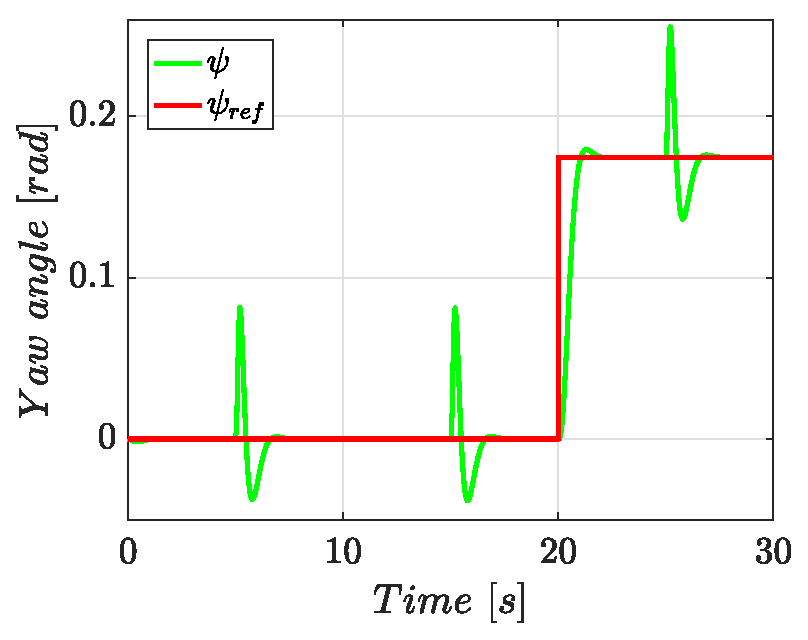
\includegraphics[width=7.0cm]{althold_psi_lqi}
\caption{Rotation about $y$ axis, $J_{yy}$ experiment}
\label{fig:althold_psi_lqi}
\end{subfigure}\\[1ex]
\begin{subfigure}{0.5\linewidth}
\centering
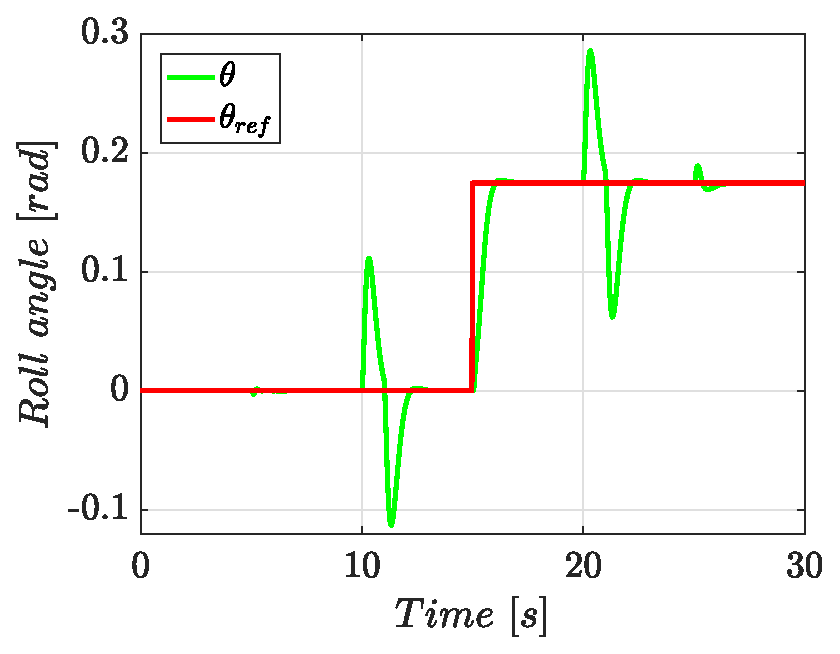
\includegraphics[width=7.0cm]{althold_theta_lqi}
\caption{Rotation about $z$ axis, $J_{zz}$ experiment}
\label{fig:althold_theta_lqi}
\end{subfigure}
\begin{subfigure}{0.5\linewidth}
\centering
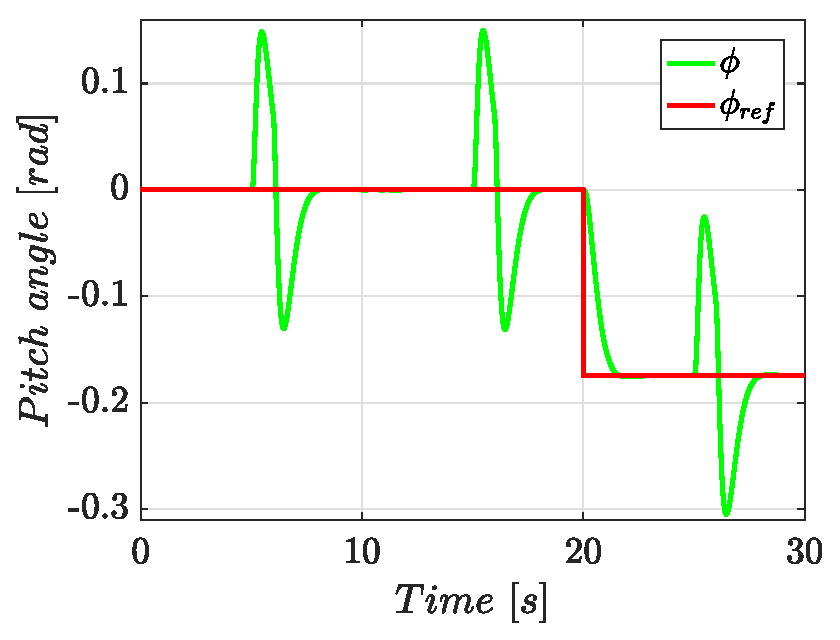
\includegraphics[width=7.0cm]{althold_phi_lqi}
\caption{Rotation about $z$ axis, $J_{zz}$ experiment}
\label{fig:althold_phi_lqi}
\end{subfigure}
\caption{Rotation about $x$, $y$ and $z$ axes during the bifilar pendulum experiments}
\label{fig:althold_lqi}
\end{figure}

\subsection{GNSS-Dependent Modes (H$_\infty$)}
\begin{figure}[h]
	\begin{center}
	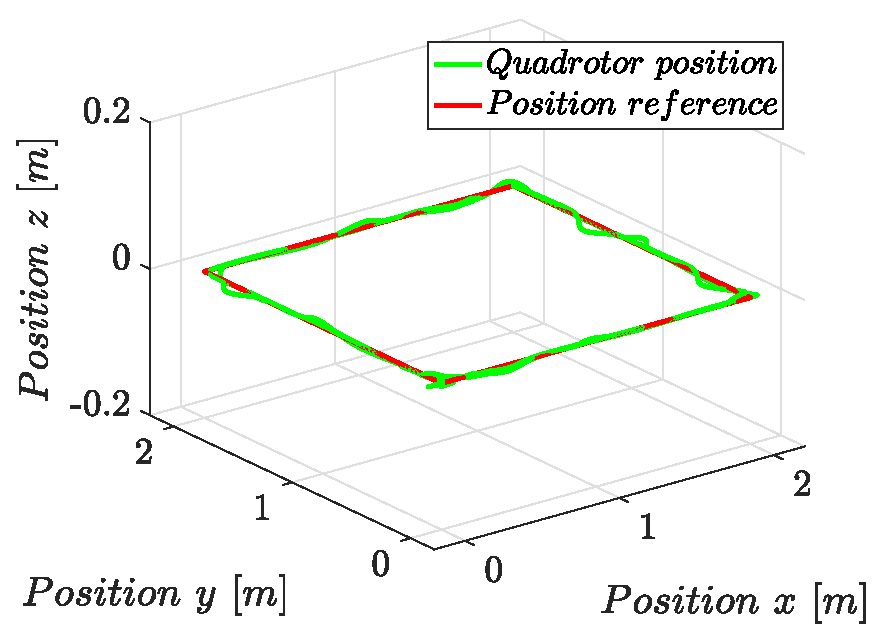
\includegraphics[width=0.8\textwidth]{auto_xyz_lqi}
	\caption{Closed-loop of the controlled system with an $H_{\infty}$ controller.}
	\label{fig:auto_xyz_lqi}
	\end{center}
	\end{figure}
	
\begin{figure}[H]
\begin{subfigure}{.5\linewidth}
\centering
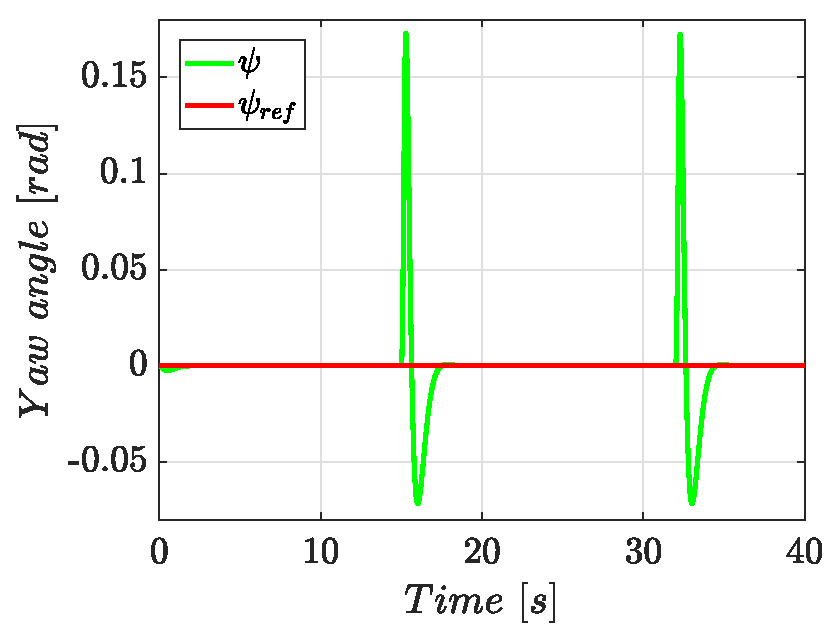
\includegraphics[width=7.0cm]{auto_psi_lqi}
\caption{Rotation about $x$ axis, $J_{xx}$ experiment}
\label{fig:auto_psi_lqi}
\end{subfigure}%
\begin{subfigure}{.5\linewidth}
\centering
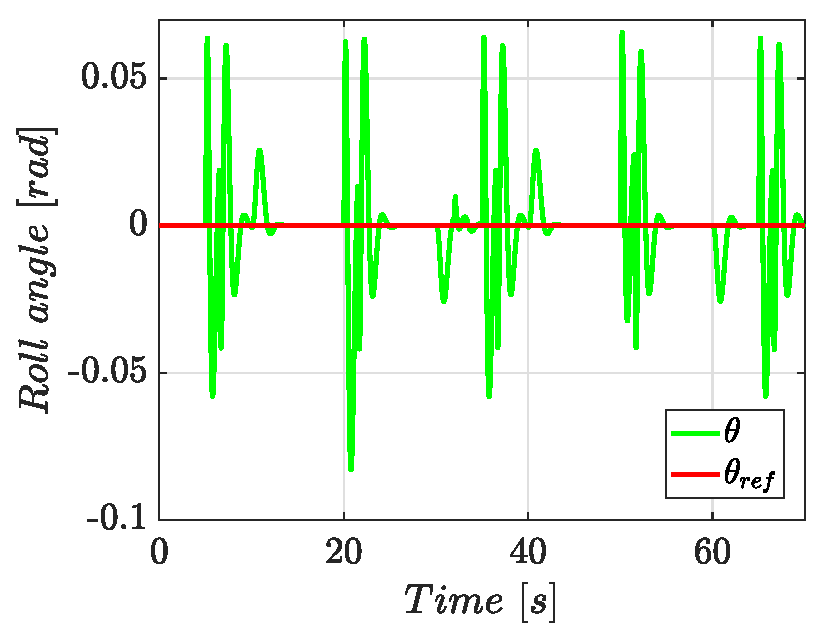
\includegraphics[width=7.0cm]{auto_theta_lqi}
\caption{Rotation about $y$ axis, $J_{yy}$ experiment}
\label{fig:auto_theta_lqi}
\end{subfigure}\\[1ex]
\begin{subfigure}{\linewidth}
\centering
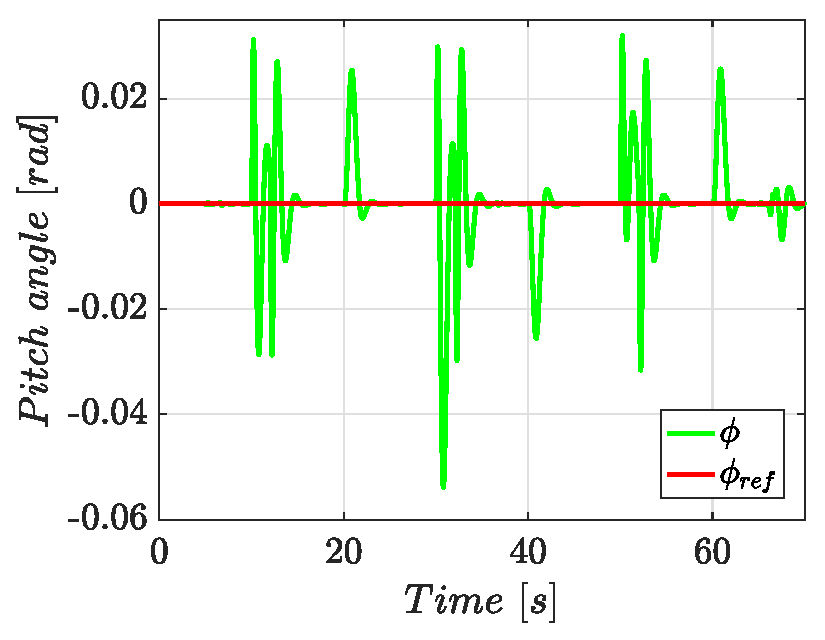
\includegraphics[width=7.0cm]{auto_phi_lqi}
\caption{Rotation about $z$ axis, $J_{zz}$ experiment}
\label{fig:auto_psi_lqi}
\end{subfigure}
\caption{Rotation about $x$, $y$ and $z$ axes during the bifilar pendulum experiments}
\label{fig:auto_lqi}
\end{figure}

\begin{figure}[h]
	\begin{center}
	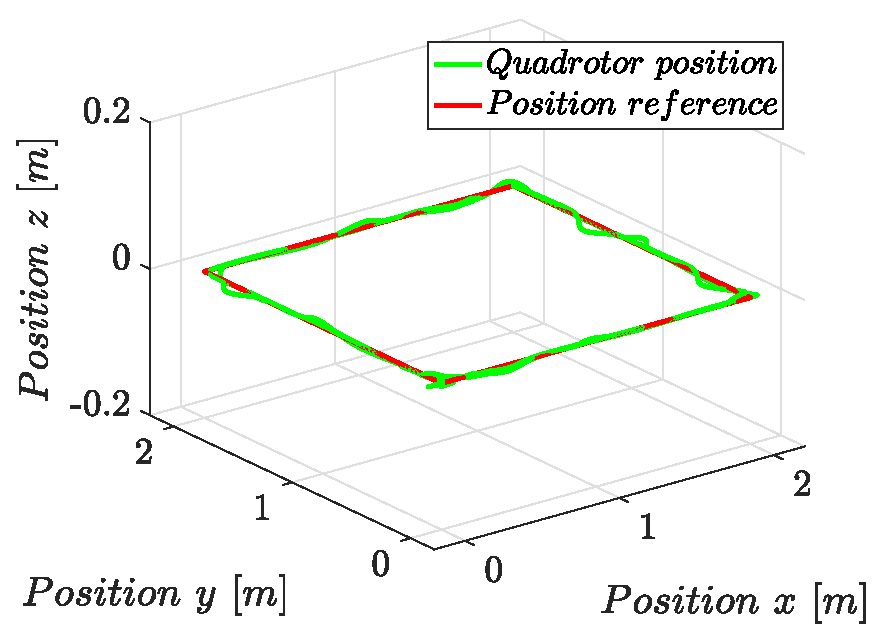
\includegraphics[width=0.8\textwidth]{auto_xyz_lqi}
	\caption{Closed-loop of the controlled system with an $H_{\infty}$ controller.}
	\label{fig:auto_xyz_lqi}
	\end{center}
	\end{figure}
	
\begin{figure}[H]
\begin{subfigure}{.5\linewidth}
\centering
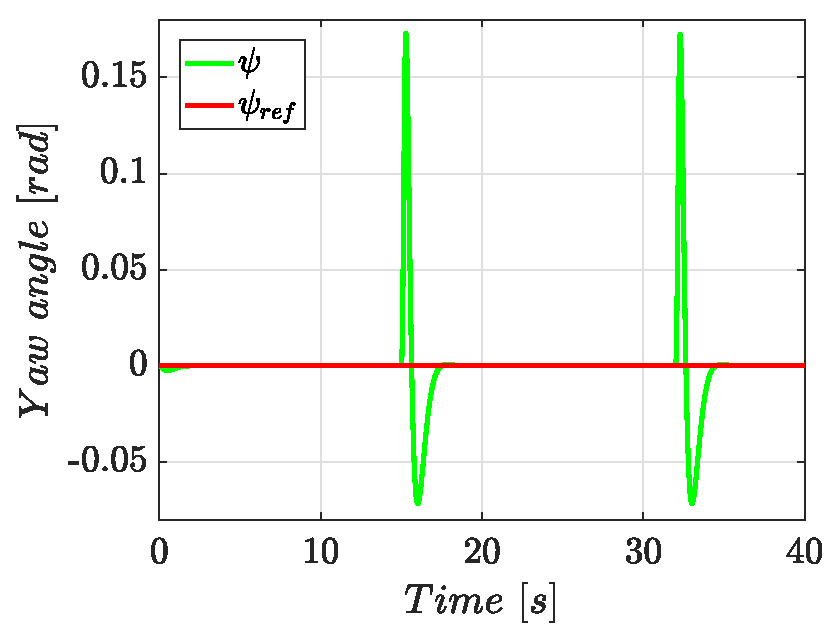
\includegraphics[width=7.0cm]{auto_psi_lqi}
\caption{Rotation about $x$ axis, $J_{xx}$ experiment}
\label{fig:auto_psi_lqi}
\end{subfigure}%
\begin{subfigure}{.5\linewidth}
\centering
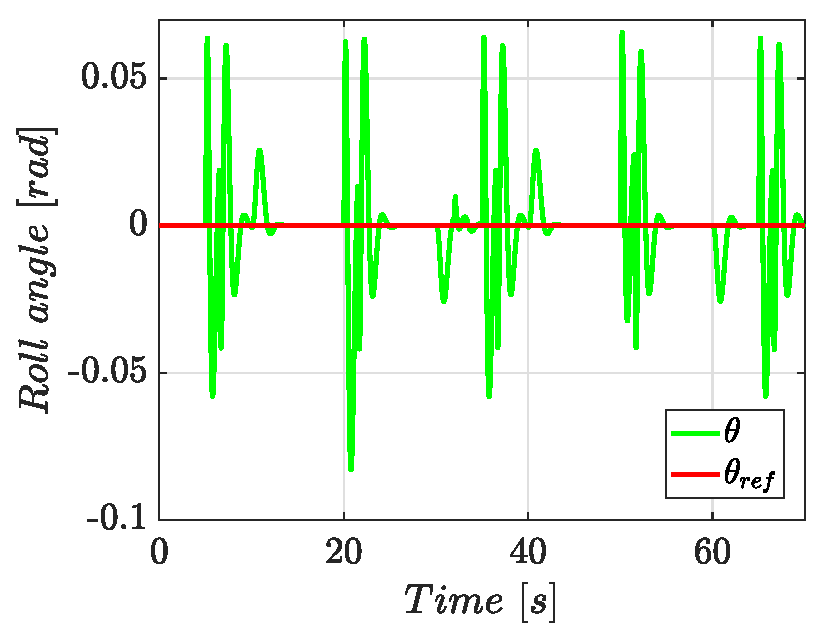
\includegraphics[width=7.0cm]{auto_theta_lqi}
\caption{Rotation about $y$ axis, $J_{yy}$ experiment}
\label{fig:auto_theta_lqi}
\end{subfigure}\\[1ex]
\begin{subfigure}{\linewidth}
\centering
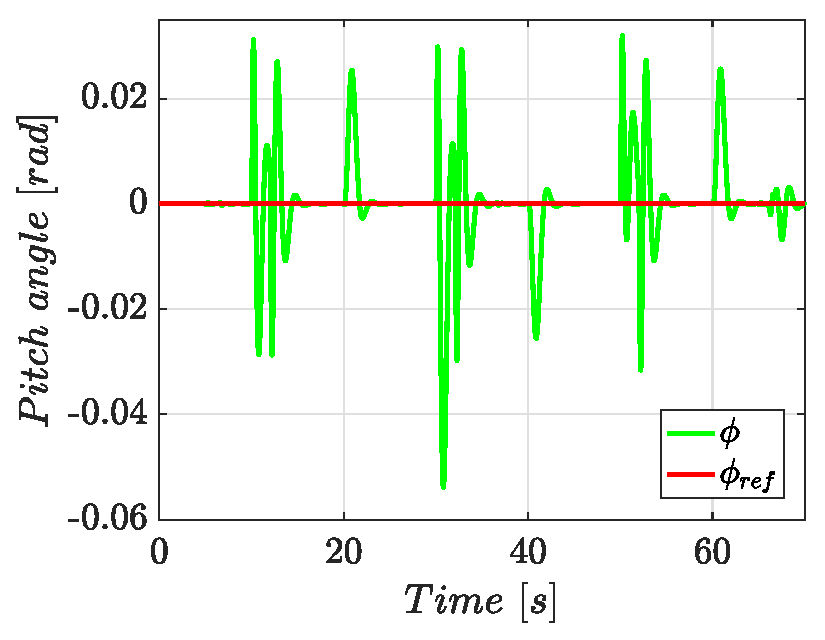
\includegraphics[width=7.0cm]{auto_phi_lqi}
\caption{Rotation about $z$ axis, $J_{zz}$ experiment}
\label{fig:auto_psi_lqi}
\end{subfigure}
\caption{Rotation about $x$, $y$ and $z$ axes during the bifilar pendulum experiments}
\label{fig:auto_lqi}
\end{figure}

\section{Conclusions}
rgrgrgtrgrtgr